\documentclass[11pt,a4paper]{article}

\usepackage[margin=1in]{geometry}
\usepackage[T1]{fontenc}
\usepackage[utf8]{inputenc}
\usepackage{lmodern}
\usepackage{microtype}
\usepackage{amsmath}
\usepackage{amssymb}
\usepackage{booktabs}
\usepackage{array}
\usepackage{longtable}
\usepackage{enumitem}
\usepackage{xcolor}
\usepackage{hyperref}
\usepackage{tikz}
\usetikzlibrary{arrows.meta,positioning,shapes.geometric}

\hypersetup{
  colorlinks=true,
  linkcolor=blue,
  citecolor=blue,
  urlcolor=blue,
  pdftitle={The Guardianship Doctrine: General Admissibility Architecture},
  pdfsubject={Normative governance architecture for reasoning under uncertainty}
}

\title{\textbf{The Guardianship Doctrine}\\[0.5em]
\large General Admissibility Architecture\\
A Normative Systems Framework for Force, Uncertainty, and Care}
\author{}
\date{Version 2.0}

\newcommand{\shall}{\textbf{SHALL}}
\newcommand{\shallnot}{\textbf{SHALL NOT}}
\newcommand{\should}{\textbf{SHOULD}}
\newcommand{\may}{\textbf{MAY}}

\begin{document}

\maketitle
\tableofcontents
\newpage

\section{Executive Summary}

The General Admissibility Architecture is a domain-independent governance framework for reasoning under uncertainty. It separates observation, inference, evidence maturity, claim maturity, model governance, and decision governance into distinct layers. The architecture is designed to prevent premature escalation from interesting observations to accepted claims, model revision, or operational action.

The framework is governed by eight constitutional invariants: admissibility before execution, authority contraction under degradation, layer independence, recovery ceiling enforcement, explicit gap labelling, provenance fixity, fail-closed default, and the principle that observability does not imply admissibility.

Evidence Quality Weight (EQW) v1.1 and the Theory Revision and Admissibility Architecture (TRAA) are included as informative reference implementations. They are not mandatory for conformance. A conforming system may use alternative evidence-quality or claim-assessment methods, provided that the normative layer contracts and governance invariants are satisfied.

\section{Introduction}

\subsection{Purpose}

This document defines a normative architecture for governing the progression from raw observations to operational decisions. Its central purpose is to ensure that increasing confidence, visibility, or analytical sophistication does not silently expand authority.

\subsection{Scope}

The architecture applies to scientific, engineering, medical, computational, legal, safety, and governance contexts. It is not a theory of truth and does not prescribe one universal scoring system. It defines the conditions under which artifacts may progress between governance layers.

\subsection{Normative and Informative Material}

Sections describing the architecture, governance invariants, layer contracts, state transitions, audit obligations, and conformance criteria are normative. Sections describing EQW, TRAA, examples, calibration, and literature foundations are informative unless explicitly stated otherwise.

\section{General Admissibility Architecture}

\subsection{Definition of Admissibility}

Admissibility is the property that an artifact satisfies the entry criteria required to progress from one governance layer to the next.

Each layer \shall define:

\begin{itemize}[leftmargin=*]
  \item required inputs;
  \item permitted processes;
  \item required outputs;
  \item admission criteria;
  \item prohibited operations; and
  \item audit obligations.
\end{itemize}

\subsection{Layered Governance Stack}

The architecture contains six layers:

\begin{enumerate}[leftmargin=*]
  \item Observation;
  \item Inference;
  \item Evidence Maturity;
  \item Claim Maturity;
  \item Model Governance; and
  \item Decision Governance.
\end{enumerate}

\begin{center}
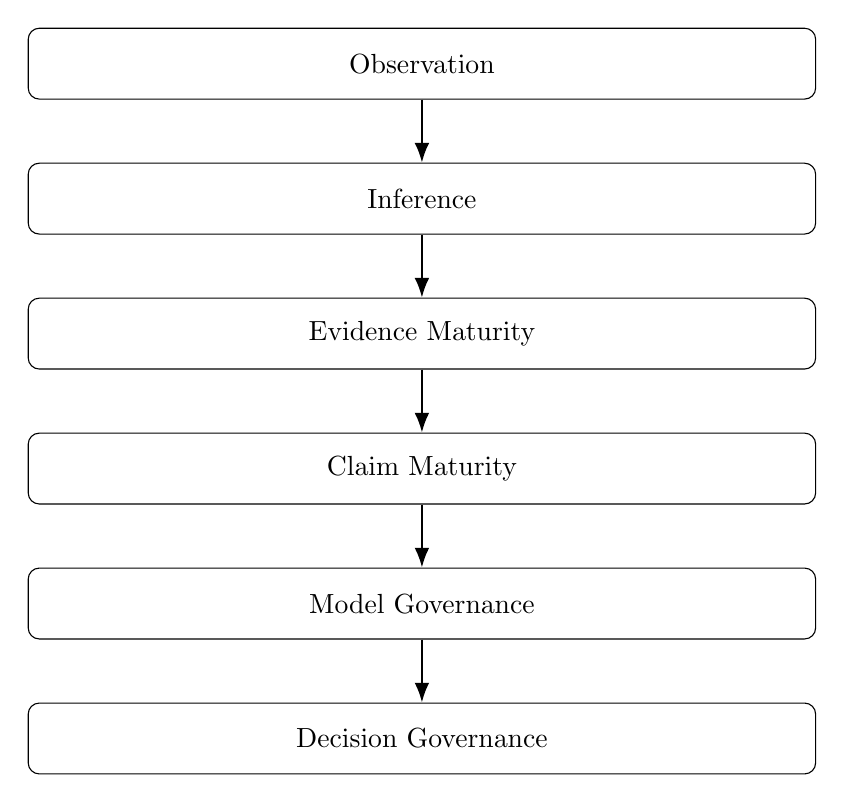
\begin{tikzpicture}[
  node distance=8mm,
  box/.style={rectangle,draw,rounded corners,minimum width=10cm,minimum height=9mm,align=center},
  arrow/.style={-{Latex[length=2.5mm]},thick}
]
  \node[box] (o) {Observation};
  \node[box,below=of o] (i) {Inference};
  \node[box,below=of i] (e) {Evidence Maturity};
  \node[box,below=of e] (c) {Claim Maturity};
  \node[box,below=of c] (m) {Model Governance};
  \node[box,below=of m] (d) {Decision Governance};
  \draw[arrow] (o) -- (i);
  \draw[arrow] (i) -- (e);
  \draw[arrow] (e) -- (c);
  \draw[arrow] (c) -- (m);
  \draw[arrow] (m) -- (d);
\end{tikzpicture}
\end{center}

\subsection{Independence Principle}

The layers \shallnot collapse into a single score, state, or decision.

The following implications are invalid unless separately justified:

\begin{itemize}[leftmargin=*]
  \item high posterior probability does not imply high evidence maturity;
  \item high evidence maturity does not imply high claim maturity;
  \item high claim maturity does not imply model revision; and
  \item model revision does not imply operational action.
\end{itemize}

The critical invariant is:

\begin{quote}
Evidence maturity \shallnot imply claim maturity.
\end{quote}

\subsection{Artifact Immutability and Judgement Separation}

State and judgement \shall remain separate. A governance decision \shall create a new judgement artifact that references its inputs, applicable ruleset, evidence, rationale, outcome, and resulting state transition. Earlier artifacts \shall remain immutable.

\section{Governance Invariants}

Governance invariants are non-negotiable structural rules that must continue to hold under uncertainty, degraded evidence, or authority pressure.

\begin{longtable}{>{\raggedright\arraybackslash}p{0.23\textwidth} >{\raggedright\arraybackslash}p{0.24\textwidth} >{\raggedright\arraybackslash}p{0.43\textwidth}}
\toprule
\textbf{Invariant} & \textbf{Architecture Layer(s)} & \textbf{Enforcement Role} \\
\midrule
\endfirsthead
\toprule
\textbf{Invariant} & \textbf{Architecture Layer(s)} & \textbf{Enforcement Role} \\
\midrule
\endhead
Admissibility Before Execution & All transitions & Every progression requires an explicit admissibility check. \\
Authority Contraction Under Degradation & Evidence Maturity, Claim Maturity, Decision Governance & Reduced evidence quality, provenance, or context forces contraction rather than escalation. \\
Layer Independence & Entire stack & Prevents collapse of observation, inference, evidence maturity, claim maturity, model governance, and decision governance into one scalar or decision. \\
Recovery Ceiling Enforcement & Evidence Maturity, Claim Maturity, Model Governance & Limits reconstruction or revision without new admissible evidence. \\
Explicit Gap Labelling & Observation, Inference & Missing, degraded, or contested evidence must be recorded rather than inferred away. \\
Provenance Fixity & Observation, Evidence Maturity & Preserves immutable chain-of-custody and replayability. \\
Fail-Closed Default & Model Governance, Decision Governance & Ambiguity defaults to non-escalation, including SILENCE or PETRIFIED states. \\
Observability $\neq$ Admissibility & Entire stack & Visibility and auditability alone never authorize progression or action. \\
\bottomrule
\end{longtable}

\section{Layer Contracts}

\subsection{Observation}

\textbf{Required:} preserve raw data, provenance, timestamps, and immutability.

\textbf{Prohibited:} alteration, selective filtering, or substitution without an explicit audit record.

\textbf{Admission criteria:} sufficient metadata must exist to support methodological-quality and provenance assessment.

\textbf{Audit obligation:} complete chain-of-custody record.

\subsection{Inference}

\textbf{Required:} document assumptions, uncertainty, priors, likelihoods, transformations, and inference method.

\textbf{Prohibited:} modification of observations or representation of an inference as a final claim.

\textbf{Admission criteria:} inference must remain logically and procedurally separate from evidence-maturity assessment.

\textbf{Audit obligation:} replayable inference record.

\subsection{Evidence Maturity}

\textbf{Required:} assess evidence quality independently of claim validity, using EQW or an equivalent method.

\textbf{Prohibited:} automatic promotion of low-quality observations into claim support.

\textbf{Admission criteria:} produce a recorded evidence-maturity state and supporting rationale.

\textbf{Audit obligation:} reviewer reconciliation where practical.

\subsection{Claim Maturity}

\textbf{Required:} evaluate specific propositions against competing explanations, objections, and rebuttals.

\textbf{Prohibited:} bypass of evidence-maturity requirements.

\textbf{Admission criteria:} satisfy a declared, domain-specific proof or justification standard.

\textbf{Audit obligation:} argument graph or equivalent structured justification record.

\subsection{Model Governance}

\textbf{Required:} revise accepted models only on the basis of mature, admissible claims.

\textbf{Prohibited:} revision based solely on novelty, anomaly, or interesting observation.

\textbf{Admission criteria:} satisfy the applicable recovery ceiling and model-change policy.

\textbf{Audit obligation:} versioned model-change log.

\subsection{Decision Governance}

\textbf{Required:} consider consequence, reversibility, domain risk, capacity, values, and affected parties.

\textbf{Prohibited:} automatic escalation from scientific confidence alone.

\textbf{Admission criteria:} pass the final fail-closed check.

\textbf{Audit obligation:} documented decision rationale and risk assessment.

\section{Reference Implementations}

\subsection{Evidence Quality Weight (EQW) v1.1}

EQW is an informative reference implementation for the Evidence Maturity layer. It is not a probability of truth and is not a complete epistemology.

A reference scalar form is:

\begin{equation}
\mathrm{EQW} = MQ \times IR \times (1-AX) \times P,
\end{equation}

where:

\begin{itemize}[leftmargin=*]
  \item $MQ$ is methodological quality;
  \item $IR$ is independent replication;
  \item $AX$ is assumption burden; and
  \item $P$ is provenance integrity.
\end{itemize}

An initial configurable policy mapping is:

\begin{center}
\begin{tabular}{ll}
\toprule
\textbf{State} & \textbf{Reference range} \\
\midrule
NORMAL & $\mathrm{EQW} \geq 0.70$ \\
AMBER & $0.40 \leq \mathrm{EQW} < 0.70$ \\
SILENCE & $0.20 \leq \mathrm{EQW} < 0.40$ \\
PETRIFIED & $\mathrm{EQW} < 0.20$ \\
\bottomrule
\end{tabular}
\end{center}

These thresholds are policy parameters, not universal constants. Implementations \should calibrate them to domain risk, evidence structure, and validation data. The multiplicative form is a scoring model, not a statistical law; correlated factors should be treated explicitly.

\subsection{TRAA}

The Theory Revision and Admissibility Architecture is an informative reference implementation for the Claim Maturity layer. It evaluates claims through competing explanations, assumption disclosure, structured argumentation, rebuttal handling, and domain-specific proof standards.

TRAA \should preserve a distinction between:

\begin{itemize}[leftmargin=*]
  \item the proposition under review;
  \item supporting evidence;
  \item competing explanations;
  \item assumptions;
  \item rebuttals;
  \item burdens and standards of proof; and
  \item the resulting claim-maturity state.
\end{itemize}

\section{State Machines}

\subsection{Evidence Lifecycle}

\begin{center}
RAW $\rightarrow$ VALIDATED $\rightarrow$ REPLICATED $\rightarrow$ MULTI-SOURCE $\rightarrow$ STABLE
\end{center}

\subsection{Claim Lifecycle}

\begin{center}
PROPOSED $\rightarrow$ PLAUSIBLE $\rightarrow$ SUPPORTED $\rightarrow$ REPLICATED $\rightarrow$ ESTABLISHED
\end{center}

\subsection{Model Lifecycle}

\begin{center}
ACCEPTED $\rightarrow$ UNDER REVIEW $\rightarrow$ EXTENDED $\rightarrow$ REVISED $\rightarrow$ REPLACED
\end{center}

\subsection{Decision Lifecycle}

\begin{center}
NONE $\rightarrow$ MONITOR $\rightarrow$ CAUTION $\rightarrow$ ACT $\rightarrow$ COMPLETE
\end{center}

Every state transition \shall emit an immutable decision record. State transitions \shallnot overwrite prior artifacts.

\section{Worked Examples}

\subsection{Astrobiology}

An infrared excess may be well observed and independently reproduced while an artificial-origin claim remains immature. The proper governance outcome may therefore be mature evidence of an anomaly, low claim maturity for an artificial explanation, no model revision, and a follow-up decision only.

\subsection{Medicine}

A biomarker may have strong analytical validity while the claim that it improves patient outcomes remains provisional. Evidence maturity and claim maturity must be governed separately, and guideline revision must remain a distinct model-governance decision.

\subsection{Particle Physics}

A detector excess may be statistically interesting without being independently replicated. The architecture permits continued data collection while blocking premature model revision.

\subsection{AI Safety}

A reproducible model-behaviour anomaly may justify monitoring or restricted deployment even while the causal explanation remains uncertain. Decision governance may contract authority on risk grounds without pretending that the scientific claim is settled.

\subsection{Engineering}

A reliable sensor anomaly may trigger a precautionary operational response when consequences are severe and reversibility is low. Such action is a risk-governance decision, not proof that a particular failure mechanism is correct.

\section{Calibration and Validation}

Implementations \should validate scoring rubrics, thresholds, reviewer agreement, and transition criteria against historical cases and prospective test sets. Calibration records \shall be versioned and auditable.

Recommended validation activities include:

\begin{itemize}[leftmargin=*]
  \item inter-rater reliability testing;
  \item retrospective calibration against known outcomes;
  \item sensitivity analysis for thresholds and weights;
  \item adversarial testing for authority drift;
  \item replay testing of governance decisions; and
  \item domain-specific failure-mode analysis.
\end{itemize}

\section{Literature Foundations}

The architecture is informed by established work in Bayesian epistemology, evidence-certainty frameworks, structured argumentation, assurance cases, belief revision, philosophy of science, and decision theory. A complete bibliography is maintained in \texttt{sources.bib}.

\section{Conformance}

A system conforms to the General Admissibility Architecture if it:

\begin{enumerate}[leftmargin=*]
  \item implements the six governance layers;
  \item preserves layer independence;
  \item enforces admissibility at every transition;
  \item satisfies all Governance Invariants;
  \item implements the required Layer Contracts; and
  \item produces auditable governance records for every transition.
\end{enumerate}

EQW and TRAA are informative reference implementations, not conformance requirements. A conforming implementation may use different evidence-quality metrics or claim-assessment methods, provided that the normative contracts and invariants are satisfied.

\section{Release Status}

The normative architecture is frozen at version 2.0. Release readiness remains subject to repository-level compile, dependency, bibliography, manifest, and artifact checks.

\appendix

\section{Canonical Integration Records}

This release incorporates the following sealed integration records:

\begin{itemize}[leftmargin=*]
  \item INT-241: Normative versus reference implementation guidance;
  \item INT-242: Governance Invariants exploration;
  \item INT-243: Governance Invariants and architecture mapping;
  \item INT-244: Governance Invariants and layer contracts; and
  \item INT-245: White paper v2.0 integration and architecture freeze.
\end{itemize}

\section{Release Gate}

The release status is READY only when:

\begin{verbatim}
placeholder_count = 0
latex_compile = PASS
pdf_exists = true
manifest_complete = true
dependency_check = PASS
\end{verbatim}

Otherwise the release status is BLOCKED.

\bibliographystyle{plain}
\bibliography{sources}

\end{document}
